\documentclass[12pt]{article}

% Packages for math and formatting
\usepackage{amsmath}
\usepackage{amssymb}
\usepackage{amsthm}
\usepackage{mathrsfs}
\usepackage{geometry}
\usepackage{fancyhdr}
\usepackage{graphicx}
\usepackage{setspace}
\usepackage{listings}
\usepackage{xcolor}

\lstset{ %
    language=Matlab,                % 语言选择
    basicstyle=\ttfamily\small,     % 字体样式和大小
    keywordstyle=\color{blue},      % 关键字的颜色
    commentstyle=\color{gray},      % 注释的颜色
    stringstyle=\color{red},        % 字符串的颜色
    numbers=left,                   % 行号位置 (左侧)
    numberstyle=\tiny\color{gray},  % 行号的样式
    stepnumber=1,                   % 行号增量
    numbersep=5pt,                  % 行号与代码的距离
    backgroundcolor=\color{white},  % 背景色
    showspaces=false,               % 不显示空格符
    showstringspaces=false,         % 不显示字符串中的空格符
    showtabs=false,                 % 不显示制表符
    frame=single,                   % 给代码加上边框
    tabsize=4,                      % 设置制表符宽度
    captionpos=b,                   % 标题位置
    breaklines=true,                % 自动换行
    breakatwhitespace=true,         % 只在空格处换行
    title=\lstname,                 % 显示代码名称
    escapeinside={\%*}{*)},         % 在代码中加入LaTeX指令
    morekeywords={*,...}            % 自定义更多关键词
}

\setstretch{1.2}
\setlength{\parskip}{1em}

% Geometry settings for better margins
\geometry{a4paper, margin=1in}

% Header and footer
\pagestyle{fancy}
\fancyhf{}
\fancyhead[L]{Kecai Xuan}
\fancyhead[C]{Math Homework}
\fancyhead[R]{\today}
\fancyfoot[C]{\thepage}

% Custom commands for common math symbols
\newcommand{\R}{\mathbb{R}}
\newcommand{\N}{\mathbb{N}}
\newcommand{\Z}{\mathbb{Z}}

\begin{document}

\setlength{\parindent}{0pt}

\title{AMSC660 Homework \#13}
\author{Kecai Xuan}
\date{\today}
\maketitle

\section*{Problem 1}

the code can be found at https://github.com/Bessgendre/homework-13-AMSC660-2024

\subsection*{(a)}

Using the Deterministic and Stochastic Nesterov method, the loss function will first increase and then decrease:
\begin{figure}[ht]
    \centering
    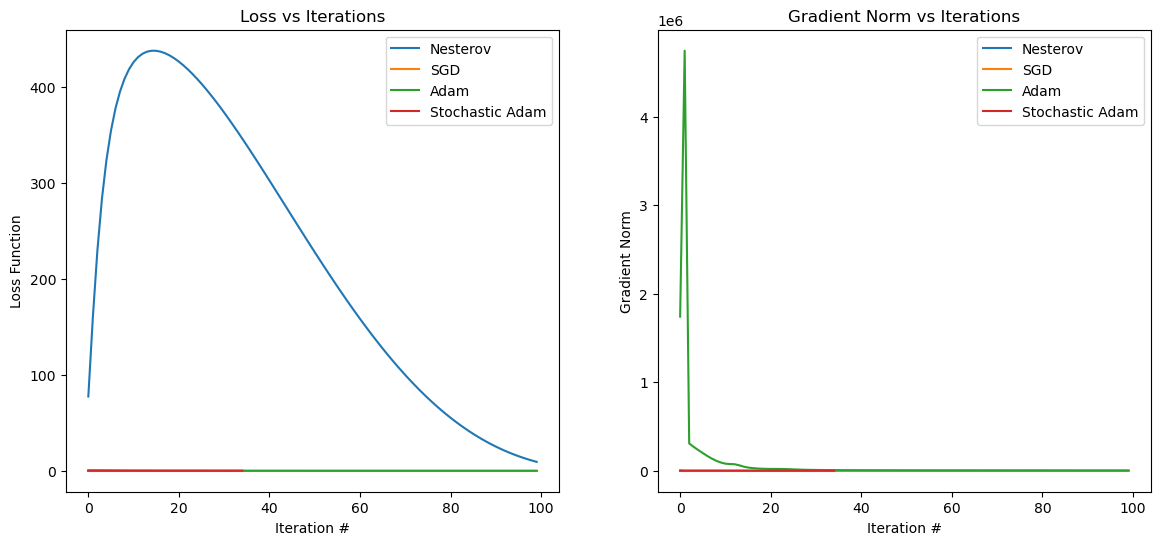
\includegraphics[width=0.8\textwidth]{./img/loss_compare.png}
\end{figure}

\subsection*{(b)}

The Stochastic Adam method is the most efficient among the four methods, with the least number of iterations and the smallest loss value:
\begin{figure}[ht]
    \centering
    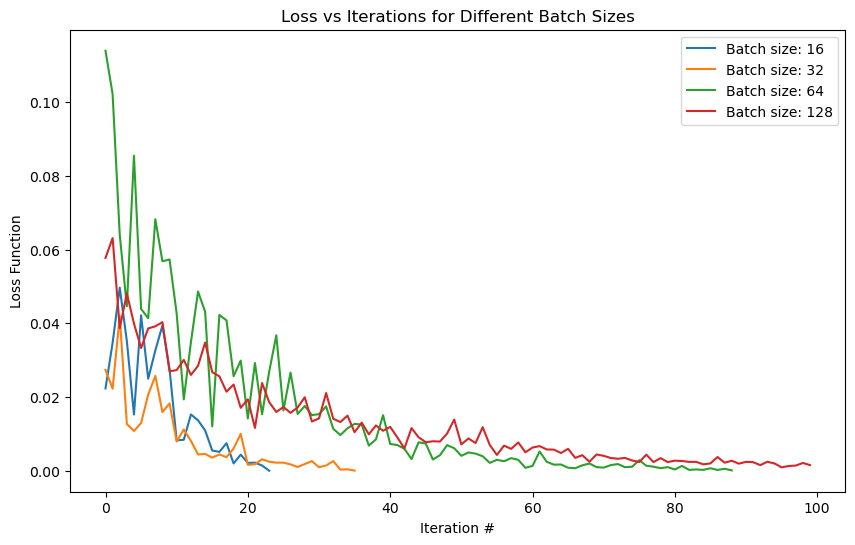
\includegraphics[width=0.8\textwidth]{./img/adam_size.png}
\end{figure}
For this problem, the best batch size is around 16.

\section*{Problem 2}

\begin{align*}
    \left[\begin{array}{cc}
        G & A^\top \\
        A & 0
        \end{array}\right]=\left[\begin{array}{cc}
        I & 0 \\
        X & I
        \end{array}\right]\left[\begin{array}{cc}
        G & 0 \\
        0 & S
        \end{array}\right]\left[\begin{array}{cc}
        I & X^\top \\
        0 & I
    \end{array}\right]
    =
    \left[\begin{array}{cc}
        G & GX^\top \\
        XG & XGX^\top + S
    \end{array}\right]
\end{align*}
Since $G$ is symmetric, as a result:
\begin{align*}
    X = AG^{-1}, \quad S = -A G^{-1} A^\top
\end{align*}
where $S$ is the negative congruence matrix of $G^{-1}$. When the eigenvalues of $G^{-1}$ are all positive, then $S$ is symmetric negative definite with the number of negative eigenvalues equal to $m$.

Since $\displaystyle K=\left[\begin{array}{cc}
    G & A^\top \\
    A & 0
    \end{array}\right]$ and $\left[\begin{array}{cc}
        G & 0 \\
        0 & S
        \end{array}\right]$ are related by congruence, they have the same number of positive, zero and negative eigenvalues, which is the result of Sylvester's law of inertia. Therefore, matrix $K$ has $d$ positive eigenvalues and $m$ negative eigenvalues.

\section*{Problem 3}

\subsection*{(a)}

Introduce the Lagrange function for this problem:
\begin{align*}
    \mathscr{L}(x, \lambda) = \frac{1}{2}x^\top Gx + c^\top x + \lambda^\top(Ax - b)
\end{align*}
where $\lambda$  is the Lagrange multiplier. The necessary conditions for optimality are:
\begin{align*}
    \nabla_x \mathscr{L}&=G x+c+A^{\top} \lambda=0 \\
    \nabla_\lambda \mathscr{L}&=A x-b=0
\end{align*}
To write it in the matrix form:
\begin{align*}
    \left[\begin{array}{cc}
        G & A^\top \\
        A & 0
        \end{array}\right]\left[\begin{array}{c}
        x \\
        \lambda
        \end{array}\right]=\left[\begin{array}{c}
        -c \\
        b
        \end{array}\right]
\end{align*}
where the matrix on the left-hand side $\displaystyle K = \left[\begin{array}{cc}
    G & A^\top \\
    A & 0
    \end{array}\right]$ is the KKT matrix. 

\subsection*{(b)}

Consider $Kz = 0$:
\begin{align*}
    \left[\begin{array}{cc}
        G & A^\top \\
        A & 0
        \end{array}\right]\left[\begin{array}{c}
        x \\
        y
        \end{array}\right]=\left[\begin{array}{c}
        0 \\
        0
        \end{array}\right]
\end{align*}
which can be written as:
\begin{align*}
        G x+A^{\top} y=0 \\
        A x=0
\end{align*}
Since $Z$ is the basis of the null space of $A$, then $x$ can be written as the linear combination of the columns of $Z$: $x = Zv$. Substitute it into the first equation:
\begin{align*}
    GZv + A^\top y = 0
\end{align*}
Multiply $Z^\top$ on both sides, because $AZ=0$, we have:
\begin{align*}
    Z^\top GZv = 0
\end{align*}
Since $Z^\top GZ$ is positive definite with full rank, then $v = 0$. Therefore, $x = 0$.

Back to $G x+A^{\top} y=0$, we have $A^\top y = 0$. Since $A$ has full row rank, then $y = 0$. Therefore, $z = 0$ is the only solution to $Kz = 0$, which means $K$ is invertible.

\subsection*{(c)}

When $K$ is invertible, there exist unique $x^*$ and $\lambda^*$ that satisfy $\displaystyle \left[\begin{array}{cc}
    G & A^\top \\
    A & 0
    \end{array}\right]\left[\begin{array}{c}
    x \\
    \lambda
    \end{array}\right]=\left[\begin{array}{c}
    -c \\
    b
    \end{array}\right]$. Therefore, the solution to the optimization problem is unique.

\section*{Problem 4}

\subsection*{(a)}

The level sets and the feasible set is shown in the following figure shaded in green:
\begin{figure}[ht]
    \centering
    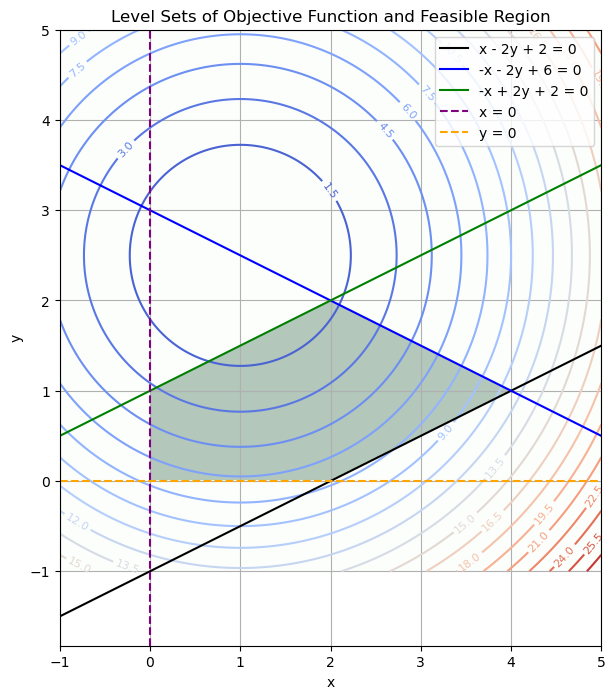
\includegraphics[width=0.5\textwidth]{./img/contour.png}
\end{figure}

\subsection*{(b)}

The feasible region is a polygon, and the level sets are  concentric circles around $(1,2.5)$. So the optimal solution should have the minimum distance to the center, which is $(1.4,1.7)$.

\subsection*{(c)}

\textbf{\large Iteration 1:}

Current iterate: $(x_1 , y_1) = (2,0)$

Active set: $\mathcal{W} = \{3,5\}$

\textbf{Step 1:} Form KKT conditions with current active set

We treat constraints 3 and 5 as equalities. Define the gradients:
\begin{align*}
        & \nabla f(x, y)=(2(x-1), 2(y-2.5)),\; \text { At }(2,0): \;\nabla f=(2(2-1), 2(0-2.5))=(2,-5) \\
        & \nabla g_3=\nabla(-x+2 y+2)=(-1,2) \\
        & \nabla g_5=\nabla(y)=(0,1)
\end{align*}
The KKT system for an active-set QP at a stationary point requires:
\[
    \nabla f(x, y)+\lambda_3 \nabla g_3+\lambda_5 \nabla g_5=0
\]
and the active constraints $g_3(x, y)=0, g_5(x, y)=0$.

Substitute:
\[
    (2,-5)+\lambda_3(-1,2)+\lambda_5(0,1)=(0,0) \quad \Rightarrow \quad \lambda_3=2, \;\lambda_5=1
\]
No search direction was needed here because we directly solved the KKT conditions at the given point. Since $\lambda_3, \lambda_5 > 0$, $(2,0)$ is a KKT point for the subproblem defined by these two active constraints, but it is not the global minimum.

Now we should drop constraint \#5 from the working set.

\textbf{\large Iteration 2:}

\textbf{Step 1:}  Compute gradient at $(2,0)$
\[
    \nabla f(x, y)=(2(x-1), 2(y-2.5)), \text { At }(2,0): \nabla f=(2(2-1), 2(0-2.5))=(2,-5)
\]

\textbf{Step 2:}  Set up KKT with active set $\mathcal{W}=\{3\}$

We must find a search direction $d = (d_x, d_y)$ that satisfies:
\[
    2\left(d_x, d_y\right)+(2,-5)+\lambda_3(-1,2)=0 \quad \text { and } \quad(-1,2) d=0
\]
where we find $d = (0.2,0.1)$.

\textbf{Step 3:}  Perform line search

We increase $\alpha$ from $0$ until another constraint becomes active or we hit the minimum along that line. After checking feasibility, no immediate blocking constraints appear for small $\alpha$. The best step (from a simple analytic line search) is found by minimizing $f$ along the direction and it comes out $\alpha = 1$ .

\textbf{Step 4:}  Update iterate
\[
    (x_2, y_2)=(2,0)+1(0.2,0.1)=(2.2,0.1)
\]

\vspace{1cm}

\textbf{\large The following iterations are similar to iteration 1 and 2. }

\vspace{1cm}

\textbf{\large Iteration 3:}

Still active set $\mathcal{W}=\{3\}$ at $(2.2,0.1)$.

No descent direction is found, $\lambda_3 = 2.4 > 0$.

Drop constraint \#3.

\textbf{\large Iteration 4:}

Unconstrained direction $d = (-1.2,2.4)$.

Move to $(1.4,1.7)$.

\textbf{\large Iteration 5:}

This is the known optimal solution. No further improvement.

\begin{figure}[ht]
    \centering
    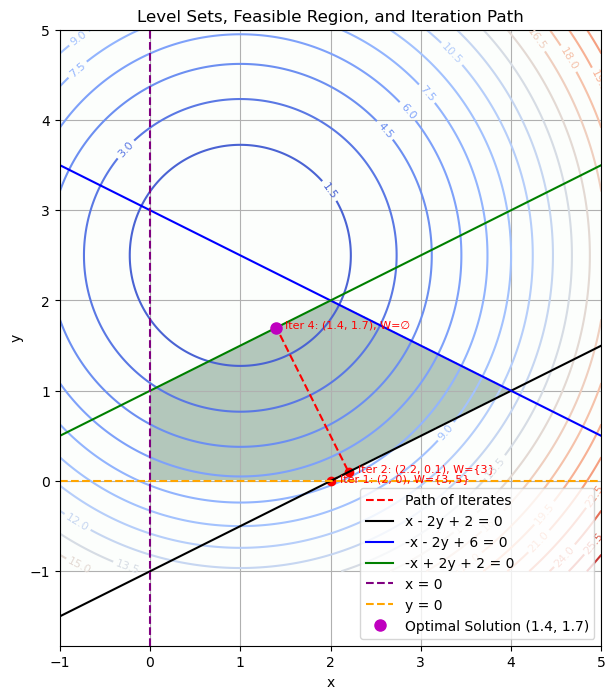
\includegraphics[width=0.6\textwidth]{./img/iteration.png}
\end{figure}




\end{document}
